% Chapter1 前端架构细节

\subsection{模块化的前端开发}

\indent
说起模块化,也许首先想到的就是编程中的模块设计,以功能块为单位进行程序设计,最后通过模块的选择和组合构成最终产品。把这种思想运用到页面构建中,也已经不是什么新鲜事。很大一部分页面架构师都经历了这样几个阶段:第一阶段是在一个css文件中把多个页面按自己的习惯顺序从上往下编写样式,基本不考虑有无公用样式,以完成设计呈现为首要目的;第二阶段是提取不同页面中的通用样式,如公用颜色、图标、按钮等,实现一些基本元素的复用;第三阶段是提取公用功能模块,如导航、版权信息等,实现部分公用模块的复用。

\indent
刚才描述的第三阶段的方法已经包含了模块化思想,不少团队也都有一套成熟的模块化开发方案。某些产品中要求使用一种称为UIO方式,模块化通用的功能模块或组件,以达到最大程度的模块独立性与复用性,过去很多工程师认为这种工作方式约束了编码的自由性,过多的结构约束反而降低了工作效率,加之产品之间也存在不统一,最后并没有运用到整个团队。

\indent
有一篇关于面向对象CSS的文章中指出,面向对象的CSS有两个主要原则:separate the structure from the skin,separate the container from the content。第一个原则体现在模块化思想可以理解为,模块的设计制作和布局框架本身相分离,意味着模块不能只为某个布局而编写样式,像存在换肤功能的产品更是如此,如果模块在不同的皮肤样式下需要另写很多样式甚至是修改结构的时候,这个模块的制作就是失败的;第二个原则说的布局与内容的分离,布局中某个位置不必只能放置某种内容,反过来可以理解为模块的灵活性和复用性。

\indent
另外,随着web应用不断发展和对JavaScript依赖的进一步加深,出现了使用模块(Modules)来组织代码和依赖性。模块使得我们创建明确清晰的组件和接口,这些组件和接口能够很容易的加载并连接到其依赖组件。 AMD模块系统提供了使用JavaScript模块来构建Web应用的完美方式,并且这种方式具有形式简单,异步加载和广泛采用的特点。

\textbf{模块系统}
\par
异步模块定义(AMD)格式是一套API,它用于定义可重用的并能在多种框架使用的模块。开发AMD是为了提供一种定义模块的方式,这种方式可以使用原生的浏览器脚本元素机制来实现模块的异步加载。AMD API由2009年Dojo 社区的讨论中产生,然后移动到讨论CommonJS如何更好的为浏览器适应CommonJS模块格式(被NodeJS使用)。 CommonJS已经发展成为单独的一个标准并有其专门的社区。

\indent
模块化系统的基础前提是:
\begin{itemize}
	\item 允许创建被封装的代码片段,也就是所谓的模块
	\item 定义本模块与其他模块之间的依赖
	\item 定义可以被其他模块使用的输出的功能
	\item 谨慎的使用这些模块提供的功能
\end{itemize}

\indent
ADM与CommonJS都满足以上需求,并将依赖模块设置为其回调函数的参数从而实现在模块代码被执行前异步的加载这些依赖模块。

\indent
AMD格式提供了几个关键的好处。首先,它提供了一种紧凑的声明依赖的方式。通过简单的字符串数组来定义模块依赖,使得开发者能够花很小的代价轻松列举大量模块依赖性。

\indent
AMD帮助消除对全局变量的需求。 每个模块都通过局部变量引用或者返回对象来定义其依赖模块以及输出功能。因此,模块不需要引入全局变量就能够定义其功能并实现与其他模块的交互。AMD同时是“匿名的”,意味着模块不需要硬编码指向其路径的引用, 模块名仅依赖其文件名和目录路径,极大的降低了重构的工作量。

\indent
通过将依赖性映射为局部变量, AMD鼓励高效能的编码实践。如果没有AMD模块加载器,传统的JavaScript代码必须依赖层层嵌套的对象来“命名”给定的脚本或者模块。如果使用这种方式,通常需要通过一组属性来访问某个功能,这会造成全局变量的查找和众多属性的查找,增加了额外的开发工作同时降低了程序的性能。通过将模块依赖性映射为局部变量,只需要一个简单的局部变量就能访问某个功能,这是极其快速的并且能够被JavaScript引擎优化。

\textbf{ADM的局限}
\par
AMD为我们提供了一个模块加载并协同工作的重要层面。然而,AMD仅仅是模块定义。它并不能为模块创建的API开出任何通用的“特别处方”。比如,你不能指望模块加载器给你提供查询引擎,并期望它从一堆可替换的查询模块中给你返回一个通用的API。当然定义这样的API更利于模块交互,但这不在AMD的范畴内。大多数模块加载器不支持将模块标识映射到不同的路径,因此如果你有可替换的模块,你最好自己定义一个模块标识到不同目标路径的映射来解决这一点。

\subsection{前端UI库——bootstrap.js}

\indent
Web前端开发者每天都与HTML、CSS、JavaScript打交道,然而不少人都是周而复始地写模板、样式和交互效果,并没有想过如何将这些重复的工作整合在一起。Twitter推出的Bootstrap能够帮助Web前端开发者摆脱这种重复劳动。

\indent
为了应对复杂的需求,早期的Twitter前端工程师在开发网站时几乎采用了所有自己熟悉的前端库。造成了网站维护困难、扩展性不强、开发成本高等问题。此时BootStrap被提上了日程。Twitter要求前端工程师完全依靠这一单一框架进行前端开发。

\indent
Twitter 在2011年8月将其开源,并在2012年2月3日发布了2.0版。这个项目已有拥超过2万位关注者和4000个分支。 Bootstrap的设计者、著名前端工程师Mark Otto这样写道:“Bootstrap是我和Jacob Thornton编写的一个前端工具箱,目的是为了帮助设计师和Web前端开发人员快速有效地创建一个结构简单、性能优良、页面精致的Web应用。它使用 了最新的浏览器技术,可以提供精致的网页排版方式以及表单、按钮、表格、网格栅格化、导航等诸多元素。”Bootstrap的内置样式继承了Mark Otto简洁亮丽的设计风格,任何开发团队都能使用它提供的HTML模板、CSS样式和jQuery组件来布署或者重建一个外观漂亮的页面应用。

\indent
BootStrap 2在原有特性的基础上着重改进了用户的体验和交互性,比如新增加的媒体展示功能,适用于智能手机上多钟屏幕规格的响应式布局,另外新增了12款jQuery插件,可以满足Web页面常用的用户体验和交互功能。

\indent
如今的Bootstrap已包括了几十个组件,每个组件都自然地结合了设计与开发,具有完整的实例文档,定义了真正的组件和模板。无论处在何种技术水平的开发者,也无论处在哪个工作流程中,都可以使用Bootstrap快速、方便地构建开发者喜欢的应用。难能可贵的是,Bootstrap依旧本着“并行开发”、“作为产品的风格指南”和“迎合所有的技能水平”的原则帮助开发者解决实际问题,不断完善自己,吸引更多人选择Bootstrap应用于自己的项目中。

\indent
然而古人云“万物相生相克”,有好就有坏,Bootstrap也是一样。对于在国内的开发者来说,最可怕的就是IE兼容问题。目前Bootstrap对 IE6到IE8的支持都不友好。另一个缺点是,采用Bootstrap的模板,网站结构时常会显得臃肿。此外,覆盖一些样式时会造成代码冗余。但与其他前 端框架相比,我个人觉得Bootstrap的缺点仅此而以,至于其他方面希望有机会与大家一起探讨和学习。

\indent
Bootstrap是一套前端开发利器。它可以帮助我们加速项目开发,让我们身处在一个完备的系统中,拥有一致的设计和实现方法。不需要在外观上花费过多时间,使开发者能将精力集中于更重要的功能。

\indent
Bootstrap将改变我们的合作方式与开发进程,任何人都可以基于Bootstrap建立可扩展的前端工具包,或者在它的基础上启动属于自己的框架。


% 前端模块

\subsection{前端模块架构}
在开始解释前端模块之前,先通过几段简单的代码来熟悉一下SeaJS的使用方法:

\lstset{language=C}

\begin{lstlisting}[frame=single]
define(function(require, exports, module) {
	var moduleA = require('A');		
	exports.ret = moduleA;
}
\end{lstlisting}
\indent
上面的代码用于定义一个模块,其中require是一个方法,用来获取其他的模块,如:require('A'),exports是一个输出对象,相当于return关键字。


\lstset{language=C}

\begin{lstlisting}[frame=single]
seajs.use(['moduleA'], function(A) {
	A;
})
\end{lstlisting}
\indent
这段代码演示了如何使用定义好的模块,但它一般在初始化才被使用,其他方式都是通过在其他定义(define)模块中使用require方法来实现。

\subsubsection{初始化Javascript模块}
在请求一个页面后,默认载入位于根目录下assets/scripts/index.js模块,不过可以通过在视图页如下声明来改变初始化的Javascript模块:

\lstset{language=lisp}

\begin{lstlisting}[frame=single]
block Module
	script(src='/scripts/pages/issue.js')
\end{lstlisting}

\noindent
下面列出assets/scripts下主要文件或文件夹的作用:
\begin{description}
	\item[sea-config.js] seajs的配置模块
	\item[index.js] 默认的初始化模块
	\item[lib] 浏览器端需要用到的Javascript类库
	\item[utils] 工具模块组,多用于兼容浏览器、独立不依赖于大量css的UI模块等
	\item[widgets] 大型UI组件,依赖大量的css样式以及模版(html/jade/...)
	\item[pages] 与视图(view)所对应的初始化模块
\end{description}

\subsubsection{视图}
所有的视图都位于根目录下的views下,views/shared用于存放公用的视图。系统内所有的模版都是使用一个名为Jade的模版语法书写的。

\textbf{Jade/Haml}
\par
Jade是一款高性能简洁易懂的模板引擎,Jade是Haml的Javascript实现,在服务端(NodeJS)及客户端均有支持。

\indent
Haml是一种用来描述XHTML web document的标记语言,它是干净,简单的。而且也不用内嵌代码。Haml的职能就是替代那些内嵌代码的page page templating systems,比如PHP,ERB(Rails的模板系统),ASP。不过,haml避免了直接书写XHTML代码到模板,因为它实际上是一个xhtml的抽象描述,内部使用一些代码来生成动态内容。Haml 是一种简洁优美的模板语言,可以应用于Ruby on Rails、 PHP等Web开发平台,可以大大缩减模板代码,减少冗余,提高可读性。并且Haml是一种完备的模板语言,没有牺牲当前模板语言的任何特性。Haml由Hampton Catlin发明并且开发了Ruby on Rails上的实现。

\textbf{模版依赖}
\par
Jade支持模版嵌套,通常是通过block标记来实现这一功能,这样可以大大地减少模版代码的冗余与数量,不过也相应会出现模版依赖的问题,往往在一个存在复杂视图关系的web应用中,视图会越来越复杂,也越来越难以维护。

\indent
Web开发过程中,视图通常需要经常更改,或者增加、删除。这样就需要工程师除了写好视图文件内的模版代码外,还需要考虑清楚视图文件夹(views)内的文件架构,即如何命名,如何分类视图文件、模版文件等,后者与路由(Router)设计、控制器(Controller)设计是相互依赖、相互影响的关系。

\noindent
根模版views/shared/skeleton.jade代码如下:

\lstset{language=lisp}

\begin{lstlisting}[frame=single]
doctype 5
html
  head
    block Head
      meta(name='viewport', 
      	content='width=device-width, 
      	initial-scale=1.5')
      link(rel='stylesheet', 
      	href='//stk.ikanbao.fm:3000/css/bootstrap.css')
      title login
      script
        var ENV = {}
  body
    block Content
      include header
    script(src='/scripts/lib/sea.js')
    script(src='/scripts/sea-config.js')
    block Module
      script(src='/scripts/index.js')
\end{lstlisting}

\indent
在views/shared还能发现一个名为sidebar-and-content.jade的视图文件,虽然该文件也是基于skeleton模版,不过它们的用处各不相同,sidebar-and-content用于应用中的分栏布局,比如视图文件welcomAuthenicated部分代码如下:

\lstset{language=lisp}

\begin{lstlisting}[frame=single]
// Welcome Authenticated
extend shared/sidebar-and-content
block append head
block append content
\end{lstlisting}

% 前端架构图

\subsection{前端架构图}
\begin{figure}[h]
  \centering
    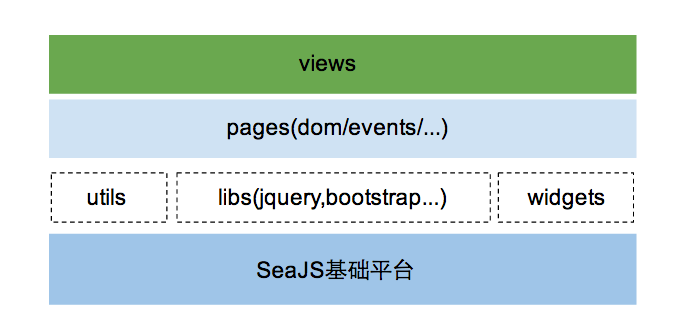
\includegraphics[width=1\textwidth]{./images/client-side-architecture.png}
  \caption{前端架构图}
\end{figure}


\clearpage